\documentclass[11pt,a4paper,twoside]{report}
\usepackage{amsmath,titlesec}
\usepackage[scaled]{beramono}
\usepackage{colortbl}
\definecolor{gray-5}{gray}{0.95}
\definecolor{gray-10}{gray}{0.9}
\definecolor{gray-20}{gray}{0.8}
\definecolor{gray-30}{gray}{0.7}
\definecolor{gray-40}{gray}{0.6}
\definecolor{fadered}{rgb}{0.8824, 0.9529, 0.8745}
\usepackage{charter}
\usepackage{longtable}
\usepackage{multirow}
\usepackage[pdftex]{graphicx}
\usepackage{caption}
\usepackage[top=1in, bottom=1in, left=1in, right=1in]{geometry}
\usepackage[charter]{mathdesign}
\usepackage[utf8]{inputenc}
\usepackage[none]{hyphenat} 
\usepackage{float}
\usepackage[final]{pdfpages}
% \usepackage{setspace}
\usepackage[charter]{mathdesign}
% \usepackage[small]{caption}
% \usepackage{abstract}
% \usepackage{lineno}

\usepackage{listings} 
\lstset{numbers=left, numberstyle=\scriptsize\ttfamily, numbersep=10pt, captionpos=b} 
\lstset{backgroundcolor=\color{gray-5}}
\lstset{basicstyle=\small\ttfamily}
\lstset{framesep=4pt}
\lstset{language={}}
\newcommand{\inlineCode}{\lstinline[basicstyle=\normalsize\ttfamily]}


\usepackage[colorlinks=true,linkcolor=black,citecolor=black,urlcolor=black,filecolor=black,bookmarks=true]{hyperref}
\hypersetup{
pdfauthor = {Michael Specht},
pdftitle = {},
pdfsubject = {},
pdfkeywords = {},
pdfcreator = {LaTeX},
pdfproducer = {pdflatex}}


    \makeatletter 
    \def\cleardoublepage{\clearpage\if@twoside \ifodd\c@page\else% 
    \hbox{}% 
    \thispagestyle{empty}
    \newpage% 
    \if@twocolumn\hbox{}\newpage\fi\fi\fi} 
    \makeatother

% Definition from latex.ltx modified
% \makeatletter
% \renewcommand*{\cleardoublepage}{%
%   \clearpage
%   \if@twoside
%     \ifodd\c@page
%       \hbox{}%
%       \newpage
%       \if@twocolumn
%         \hbox{}%
%         \newpage
%       \fi
%     \fi
%   \fi
% }
% \makeatother

\fboxsep0pt
\fboxrule0.05pt

\newcommand{\image}[5]{
  \begin{figure}[htbp]
    \centering
    \includegraphics[width=#3\textwidth]{#2}
    \caption[#5]{#4}
    \label{fig:#1}
  \end{figure}
}

\newcommand{\imageFrame}[5]{
  \begin{figure}[htbp]
    \centering
    \fbox{
      \includegraphics[width=#3\textwidth]{#2}
    }
    \caption[#5]{#4}
    \label{fig:#1}
  \end{figure}
}


\usepackage{setspace}
\usepackage{fancyhdr}
\usepackage{wrapfig}
% \renewcommand{\chaptermark}[1]{\markleft{#1}{}}
% \renewcommand{\sectionmark}[1]{\markright{#1}{}}
% \fancyhead[C]{\rightmark}
% \renewcommand{\headrulewidth}{0pt}
% \renewcommand{\footrulewidth}{0pt}
\def \cre{{\em C.~reinhardtii}}
\def \dmel{{\em D.~melanogaster}}
\def \chlre{{\em Chlamydomonas reinhardtii}}

\def \fmfour{FM4}
\def \augno{AUGUSTUS}
\def \augyes{AUGUSTUS/GPF}
\def \etal{{\em et al.}}
\def \denovo{{\em de novo}}
\def \insilico{{\em in silico}}
\def \mz{{\em m/z}}

\hyphenation{AUGUSTUS}
\setlength{\parskip}{2mm}
\setlength{\parindent}{0mm}
\renewcommand{\baselinestretch}{1.4} 
\renewcommand{\arraystretch}{1.4} 

\renewcommand{\headrulewidth}{0.25pt}

\pagestyle{fancy}

\renewcommand{\chaptermark}[1]{\markboth{#1}{}}
\renewcommand{\sectionmark}[1]{\markright{#1}}

%\setlength{\marginparwidth}{1.5cm}
%\newcommand{\note}[1]{\marginpar{\color{gray-40}\footnotesize \flushleft #1}}
\newcommand{\note}[1]{}

\newcommand{\imageCourtesy}[2]{Image courtesy of #1 \cite{#2}.}

\fancyhf{}
\fancyhead[EL,OR]{\thepage}
\fancyhead[ER]{\leftmark}
\fancyhead[OL]{\rightmark}
\fancypagestyle{plain} {
  \fancyhf{}
  \renewcommand{\headrulewidth}{0pt}
}

\lstnewenvironment{todo}{\lstset{numbers=none,frame=none,backgroundcolor=\color{fadered}}}{}
\pagestyle{empty}

% Code for creating empty pages
% No headers on empty pages before new chapter
% \makeatletter
% \def\cleardoublepage{\clearpage\if@twoside \ifodd\c@page\else
%     \hbox{}
%     \thispagestyle{plain}
%     \newpage
%     \if@twocolumn\hbox{}\newpage\fi\fi\fi}
% \makeatother \clearpage{\pagestyle{plain}\cleardoublepage}


\begin{document}
% \pagewiselinenumbers

\includepdfset{pages=-,noautoscale}

\begin{center}

\includegraphics[width=0.5\textwidth]{figures/wwu-logo-black.png}

{\Large Institut f\"ur Biologie und Biotechnologie der Pflanzen}

\vspace*{3cm}

{\bf \Huge {\em Chlamydomonas reinhardtii} from the computational proteomics perspective}

\vspace*{3cm}

{\Large Inaugural-Dissertation zur Erlangung des Doktorgrades der
Naturwissenschaften im Fachbereich Biologie der
Mathematisch-Naturwissenschaftlichen Fakult\"at der
Westf\"alischen Wilhelms-Universit\"at M\"unster}

\vspace*{2cm}

{\Large vorgelegt von}

{\LARGE \bf Michael Specht}

{\Large aus Magdeburg}

{\LARGE April 2011}

\end{center}

\cleardoublepage

\vspace*{550pt}

Dekan: Prof. Dr. Christian Kl\"ambt \newline
Erster Gutachter: Prof. Dr. Michael Hippler \newline
Zweite Gutachterin: Prof. Dr. Simone K\"onig \newline
Tag der m\"undlichen Pr\"ufung: \newline
Tag der Promotion: \newline

\cleardoublepage

\vspace*{200pt}
\begin{flushright}
{\Large\em
To my family, the great life amplifier: \\
Jule, Charlotte \& Leo
}
\end{flushright}

% \clearpage

% \begin{abstract}
% This is the abstract. Lots of hacking and MS here.
% \end{abstract}

% {\bf Abbreviations and acronyms used in the report:}
% 
% DSCAM -- down syndrome cell adhesion molecule, 
% FDR -- false discovery rate, 
% GPF -- Genomic Peptide Finder, 
% MS -- mass spectrometry,
% MS/MS -- tandem mass spectrometry,
% PSM -- peptide/spectral match

\fancypagestyle{plain}{
\fancyhf{}
\renewcommand{\headrulewidth}{0.25pt}
% \renewcommand{\footrulewidth}{0.5pt}
\fancyfoot[EL,OR]{\thepage}
\fancyhead[EL]{\leftmark}
\fancyhead[OR]{\rightmark}
}

\cleardoublepage
\setcounter{tocdepth}{2}
\setcounter{secnumdepth}{2}
\tableofcontents

\clearpage

% ==============================================================
\chapter{Introduction}
% ==============================================================

% --------------------------------------------------------------
\section{Chlamydomonas reinhardtii}
% --------------------------------------------------------------

\subsection{Anaerobic metabolism}

\subsection{Iron-deficiency}

% --------------------------------------------------------------
\section{Mass spectrometry}
% --------------------------------------------------------------

\subsection{Data acquisition}

\subsection{Data evaluation}

\subsubsection{Identification}

\subsubsection{Quantitation}

% ==============================================================
\chapter{Publications}
% ==============================================================

% \newevenside
% --------------------------------------------------------------
\section{Proteomics to go: Proteomatic enables the user-friendly creation of versatile MS/MS data evaluation workflows}
% --------------------------------------------------------------

% \cleardoublepage
% 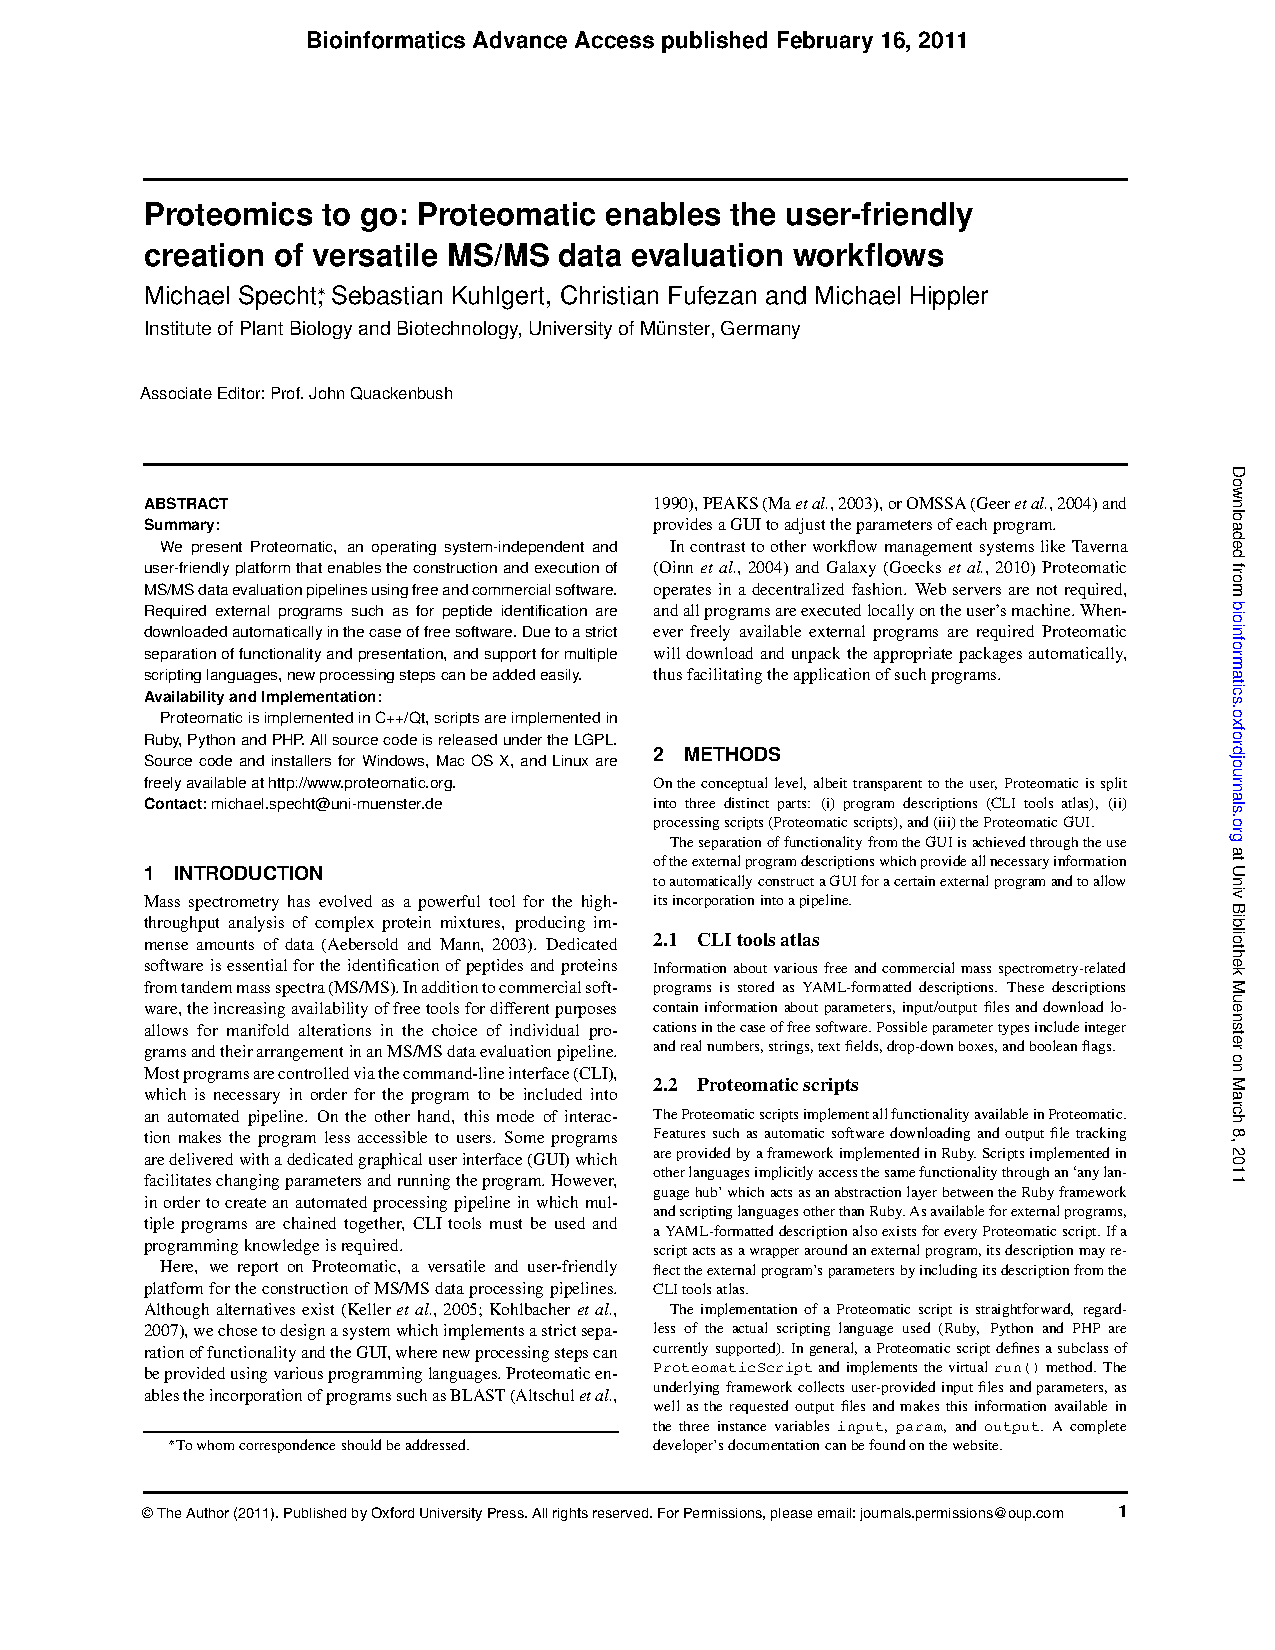
\includepdf{publications/proteomatic-2011.pdf}

% --------------------------------------------------------------
\section{qTrace: Rapid peptide and protein quantitation of metabolically labeled samples}
% --------------------------------------------------------------


% \newevenside
% --------------------------------------------------------------
\section{Characterizing the anaerobic response of Chlamydomonas reinhardtii by quantitative proteomics}
% --------------------------------------------------------------

% \newevenside
% --------------------------------------------------------------
\section{The chloroplast proteome: A concise survey form the Chlamydomonas reinhardtii perspective}
% --------------------------------------------------------------


% \newevenside
% --------------------------------------------------------------
\section{Concerted action of the new Genomic Peptide Finder and AUGUSTUS allows for automated proteogenomic annotation of the Chlamydomonas reinhardtii genome}
% --------------------------------------------------------------
% \cleardoublepage
% 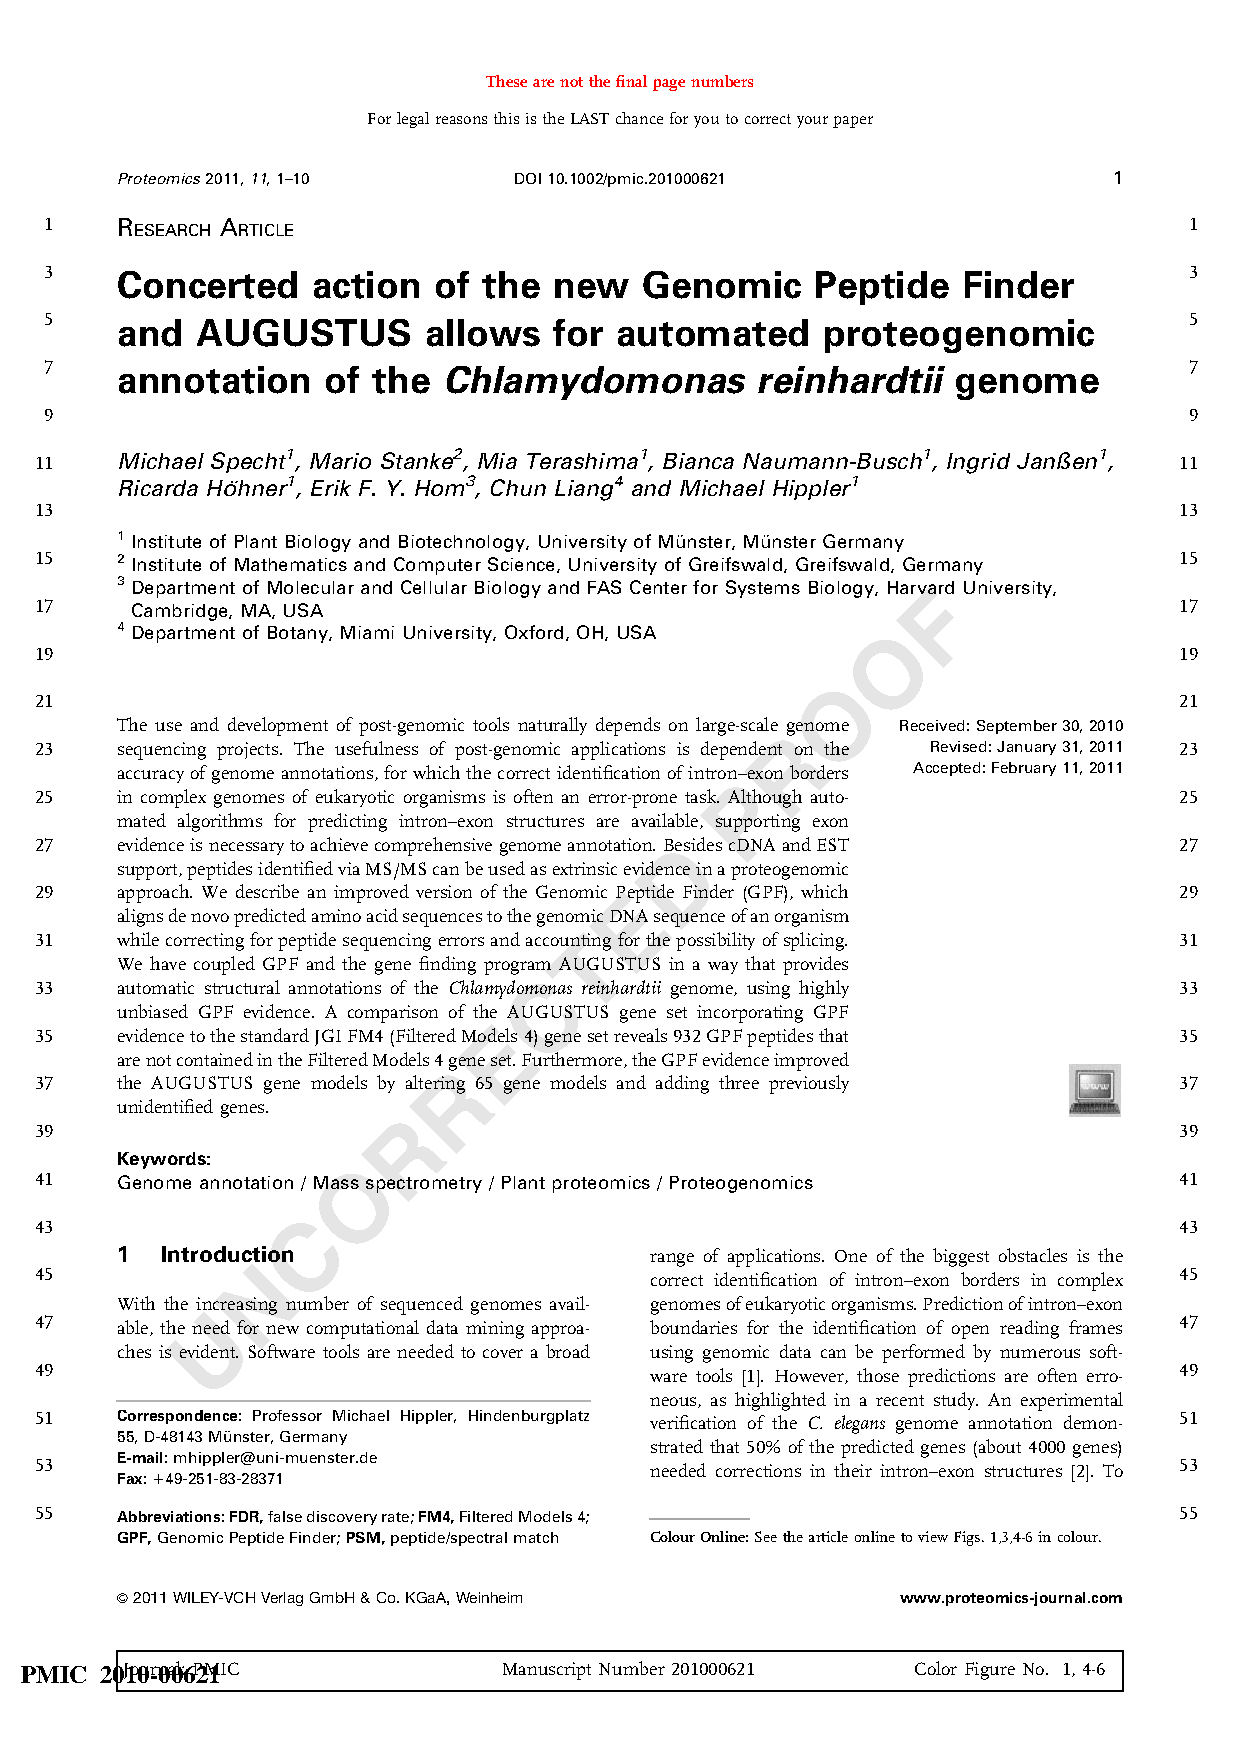
\includepdf{publications/gpf-2011.pdf}


% --------------------------------------------------------------
\section{T.~oceanica paper with Markus Lommer}
% --------------------------------------------------------------

% \newevenside
% --------------------------------------------------------------
\section{p3d -- Python module for structural bioinformatics}
% --------------------------------------------------------------

% ==============================================================
\chapter{Discussion}
% ==============================================================

Cite \cite{Specht2011}.

\bibliography{library}
\markboth{Bibliography}{Bibliography}
\bibliographystyle{unsrt}
    
\end{document}
